\section{Modélisation de l'interface graphique}

A partir du cahier des charge des l'application, j'ai construit le flowchart (\textit{représentation schématique d'un enchainement d'action}) de l'intéraction utilisateur sur les différentes pages de l'application, voir l'annexe \ref{appendix:ihm}. J'ai tout d'abord listé les différentes pages que doit composer l'application. Une page est représentée par un rectangle avec le nom de la page accompagné d'un bref déscriptif. La navigation entre deux pages est représenté par une flèche directionnel vers la page de destination avec le déclencheur qui provoque le changement de page (representé par un losange).

\begin{figure}[H]
  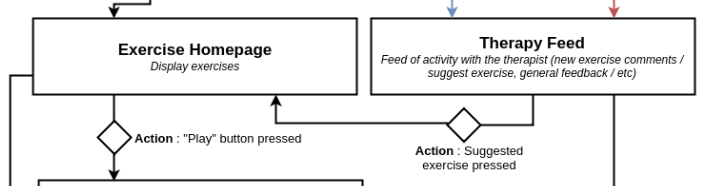
\includegraphics[width=.8\linewidth]{content/imgs/ihm_ex.png}
  \caption{Exemple du flowchart entre les pages \textit{Exercice Homepage} et \textit{Therapy Feed}}
  \label{fig:flowchart}
\end{figure}

Une fois, les différentes pages de l'application définie, je me suis attelé a faire elaboré les \textit{wireframes} de l'application. Un \textit{wireframe} est une maquette fonctionnelle, c'est à dire une representation schématique de l'interface pour définir les différents composants de l'interface sans se soucier des règles de design comme les couleurs ou la typrographie par exemple. Les \textit{wireframes} se concentrent sur l'ergonomie de l'application et non sur le desgin de celle-ci. La figure \ref{fig:wireframe} montre un exemple du \textit{wireframe} de la page principale d'un utilisateur bègue. Tous les \textit{wireframes} de l'application sont disponible dans l'annexe \ref{appendix:wireframes}.


\begin{figure}[H]
  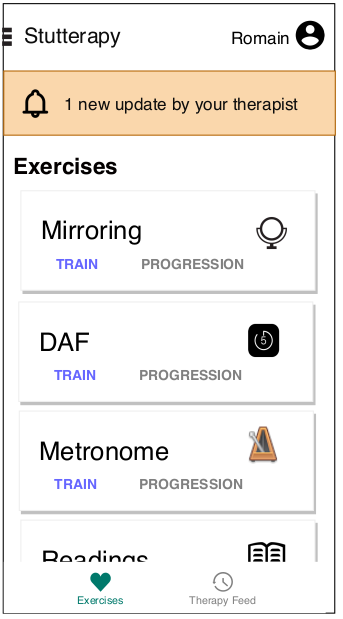
\includegraphics[width=.3\linewidth]{content/imgs/wireframe_ex.png}
  \caption{Exemple du flowchart entre les pages \textit{Exercice Homepage} et \textit{Wireframe de la page principale d'un utilisateur bègue}}
  \label{fig:wireframe}
\end{figure}
